\section{The Book of Taliesin}\label{sectiontaliesin}
This section analyses several poems from the \gls{bt} in order to present a clear picture of how lenition was represented from the sixth century onwards. The \gls{bt} is particularly suitable for this task because it not only contains a great deal of variation in age, but also because all of its contents are written by the same scribe, so scribal innovation may be supposed to have occurred in a roughly consistent manner across the various texts.  The manuscript itself dates from the beginning of the fourteenth century~\autocite[79]{huws_medieval_2000}. I will discuss \mw{Trawsganu Kynan, Armes Prydein}, and several other prophecies from the \gls{bt} in this section.


\subsection{Trawsganu Kynan}
Here, I discuss \mw{Trawsganu Kynan}, which satirises Cynan Garwyn, who most likely flourished in the second half of the sixth century. \Textcite{williams_canu_1960} dates the poem to this same period. The text has many \gls{ow} features in its orthography.  \Textcite[178]{isaac_trawsganu_1999}, however, dates it to the second quarter of the tenth century. I use Isaac's edition for line numbering in Table~\ref{trawsganukynan}


\begin{table}[h]
\centering
\begin{tabular}{@{}lllll@{}}
\toprule
\textbf{Line} & \textbf{Word} & \textbf{Translation} & \textbf{Cause of lenition} & \textbf{Represented} \\ \midrule
2 & \mw{ket} & `gift' & object lenition & no \\
11 & \mw{karrec} & `stone' & feminine noun & no \\
13 & \mw{kynan} & (personal name) & \mw{cant} & no \\
17 & \mw{Ỽy} & (place name) & \mw{ar} & yes \\
19 & \mw{ladet} & `must kill' & \mw{a} & yes \\
21 & \mw{maỽꝛ} & `large' & feminine noun & no \\
21 & \mw{tec} & `fair' & feminine noun & no \\
22 & \mw{molet} & `praise poem' & \mw{a} `from' & no \\
24 & \mw{gỽoꝛgret} & `surplus' & \mw{a} `from' & no \\
26 & \mw{gerdet} & `walk' & \mw{ar} & yes \\
27 & \mw{welet} & `see' & \mw{ry} & yes \\
28 & \mw{biỽ} & `cattle' & \mw{y} `his' & no \\
35 & \mw{gynan} & (personal name) & \mw{o} & yes \\
37 & \mw{lydan} & `broad' & feminine noun & yes \\
40 & \mw{godaran} & `noisy' & feminine noun & no \\
46 & \mw{lydan} & `broad' & feminine noun & yes \\
48 & \mw{gochvan} & `praise' & \mw{y} `his' & no \\
50 & \mw{gynan} & (personal name) & \mw{dy} `to' & yes \\ \bottomrule
\end{tabular}
\caption{Representation of lenition in \mw{Trawsganu Kynan}}
\label{trawsganukynan}
\end{table}

As can be seen in Table \ref{trawsganukynan}, lenition is only sporadically attested orthographically. This is a solid clue that a written exemplar in \gls{ow} existed to produce this text. But the orthography of \mw{Trawsganu Kynan} brings some additional clues. At one point,  \mw{l} is used for word-initial /ɬ/ in l.~20 \mw{A lafyn} `and a blade'. This betrays that lenition of this consonant was not written in an earlier version of this text. Therefore, it is misleading to regard l.~19 \mw{ladet}, l.~37 \mw{lydan}, and l.~46 \mw{lydan} as representing lenition, even though they happen to do so from a \gls{mw} synchronic point of view.

Lenition of /g/ is represented in l.~9 \mw{Ỽy} `Wye', and \mw{welet} `see;'. In these cases, the /g/ is actually an innovation, as these words go back to initial */\cw/. Some awareness of this may still have existed in the period when \mw{Trawsganu Kynan} was first written down. This makes these instances somewhat comparable to /ɬ/ being represented with a single \mw{l}.

Finally, /k/ is written lenited in the following instances: l.~26 \mw{gerdet}, l.~35 \mw{gynan}, and l.~50 \mw{gynan}. The fact that three instances of orthographic lenition are voiceless stops even though lenition is represented so scarcely shows that voiceless stops were not particularly impervious to having lenition represented. This fact, taken together with a more general tendency not to represent lenition orthographically of other consonants, brings us to the conclusion that this text had an \gls{ow}, pre-orthographic lenition exemplar, where orthographic lenition was supplied in a period when lenition of consonants including voiceless stops was written. 

In contrast to the material of the Book of Aneirin, \mw{Trawsganu Kynan} shows fairly little lenition overall: lenition is only represented orthographically in 8 out of 18 cases, which is in the same sixty-percent region we see for voiceless stops only in the Prophecies and the Book of Aneirin. However, the orthographical lenition that is supplied, is supplied to voiceless stops in roughly equal measure as it is to other consonants. This leads me to conclude that lenition was supplied to \mw{Trawsganu Kynan} at a similarly late date to when it was added to the voiceless stops of \mw{Armes Prydein} and the other prophecies.

Haycock theorises that the scribe was unfamiliar with his presumably early \gls{ow} exemplar. She notes the following: 
\tqt{The fact that he has not modernised such [Old Welsh] forms in Trawsganu Kynan Garwyn may suggest that he was not confident with Old Welsh; their infrequency elsewhere implies, then, that he was working from an exemplar or exemplars which had already been largely updated, or one(s) which contained materials which had never been written down in Old Welsh.}{haycock_legendary_2015}{7}
This same line of reasoning may be used to explain why the scribe did not bother to modernise the orthography of lenition in about half the cases: the text was simply too far removed from him. 

Incidentally, this quote also shows once more that looking at the rate at which lenition is represented may allow us to look at what kind of exemplar the scribe had before him, but if this exemplar was itself innovative in representing lenition, then a text may look younger than it is. 

\subsection{Other old poems by Taliesin}

\Textcite{williams_canu_1960} considers several more poems to be composed by the historical Taliesin, so these poems should also be as old as the late sixth century. I discuss these here.

Many of these poems have a very formulaic ending, which goes as follows\footnote{II--VII, IX from \textcite{williams_canu_1960} all have it. The example comes from VI. Translation by W.\ F.\ Skene}:

\mwcc[]{\gls{bt} p.~60, ll.~25--26}{ac yny vallỽyfy hen~|
ym dygyn agheu aghen.~|
ny bydif ym dyrwen~|
na molỽyf uꝛyen}
{And until I fail in old age,~|
In the sore necessity of death,~|
May I not be smiling,~|
If I praise not Urien. }
Now, why are \mw{bydif} and \mw{molỽyf} not lenited? The original inherited rule is that the negative particle should cause spirantisation in a main clause, and lenition in a relative clause. The MoW rule is that it should cause spirantisation where possible, and otherwise lenition. In other words, either only \mw{molỽyf} should be lenited, or both, but never neither. Also, \mw{yny} consisting of \mw{o} `if' and verbal particle \mw{ni} lenites \mw{vallỽyf}. This same distribution of lenition and non-lenition is found  in every poem which ends with this formula. 

\Textcite{strachan_mutations_1907} was the first to notice how the Early Welsh mutations following \mw{ni} and \mw{rhy} initially differed in main clauses and relative clauses. He also connects this with Old Irish preverbs that cause no mutation in main clauses, and cause lenition in relative clauses. Following \mw{ny}, Strachan finds examples of both leniting \mw{p, t, c} in relative clauses and main clauses with no lenition to other consonants. On \mw{rhy}, he notes the following: `For \textit{rhy} the evidence is less abundant, as \textit{rhy} was a disappearing particle. Confusion seems to have set in earlier than in the case of \textit{ny} ; but the facts find their simplest explanation in the same hypothesis'~\autocite[23]{strachan_mutations_1907}.

Evans gives the following description of the \gls{mw} situation:
\tqt{In the early period, the negative in a relative clause is followed by lenition of all lenitable consonants, including \textit{p, t, c} [\dots] In principal clauses, on the other hand, the negative was usually followed by the spirant mutation [\dots] In \gls{mw} prose the earlier system has been much simplified, and the position may briefly be summarized as follows: \textit{neu} and \textit{ry} are followed by lenition in every case. After the negative we have the spirant mutation of \textit{p, t, c}, and lenition of the other lenitable consonants, in both principal and relative clauses. Traces of the older construction survive in non-lenition of \textit{b} and \textit{m} after the negative [\dots]; but lenition occasionally occurs [\dots] In poetry the older system probably persisted longer. Examples of lenition of \textit{c} after the negative are found in the poetry of Dafydd ap Gwilym.
}{evans_grammar_1964}{\S65 N. 1}
It seems that the final lines of these poems are not unique in this respect. Lenition following \mw{ny} is applied to \mw{b} and \mw{m} inconsistently, even when lenition of these consonants is  represented consistently in other grammatical contexts\todo{Beth sy'n digwydd yma?}. See also Example~\ref{mwyn}, where \mw{ny byd} shows no lenition either\todo{This matter is found across \gls{mw}, and should thus be discussed in the introduction if at all.}.

Non-lenition of these consonants is found up until present-day Welsh. \Textcite{ellis_cronfa_2001}'s corpus of Welsh gives 197\footnote{197 out of 248. The other 51 were unusable, containing phrases such as \mw{ni oedd}.} valid results for \mw{ni} followed by a form of \mw{bod}. Among these, 51 did not have lenition following \mw{ni}, and the remaining 146 did. \Textcite[695]{thomas_gramadeg_1996} notes that this may be a feature of literary speech.

General failure to lenite or spirantise according to the archaic rule (spirantising in main clauses, leniting in relative clauses) may point towards a fairly late addition of lenition to the texts. The reasoning behind this is that the addition of lenition to \mw{b} and \mw{m} must postdate the collapse of the archaic mutation rule following \mw{ny}. Notably, \mw{b} and \mw{m} are both quite early in showing lenition word-initially\footnote{Lenition of these consonants is found  in texts as old as \mw{Breint Teilo}. Cf.\ the following lines from the second part: \mw{y thir hay dayr dy luyd, dy uuner (<muner), di gauayl, ha pop cyfreith a uo (<bo) dy brennin Morcannhuc yn lys} `Its lands (shall be) without military service, distraint. And every law which the king of Morgannwg may have in his court,'~\autocite[135--136]{davies_braint_1974}.\todo[inline]{Braint Teilo deserves its own section}}.

One other point that may have relevance here is that in the clause \mw{na molỽyf uꝛyen} the antecedent of the relative clause is neither the subject nor the object. In Old Irish, a non-subject and non-object antecedent of a relative verb with a negative particle would have nasalisation rather than lenition following this particle. Non-lenition here may be due to similar circumstances inherited from a common phase. 

The two poems about Gwallawg contain several instances of non-lenition after \mw{ni} and \mw{ry}: 
\begin{mwl}
\mwc[bt3011]{\gls{bt} 30.11, l.~25}{ny medylyeiſti dy alon}{You thought little of your foes; \autocite[trans.][91]{clancy_triumph_1998}}
\mwc[bt642]{\gls{bt} 64.2, l.~5}{ny golychaf an gnaỽt beird o vꝛython\footnote{\Textcite[99]{williams_canu_1960} emends \mw{ny} to \mw{ry}, which behaves the same in terms of mutations following.}}{I will praise with the song of the Britons' poets \autocite[trans.][92]{clancy_triumph_1998}}
\mwc[bt6411]{\gls{bt} 64.11--12, ll.~18--20}{rygohoyỽ rylyccraỽꝛ rylyccrer. rytharuaỽꝛ rybarnaỽꝛ. rybarn paỽb ygỽr banher}{The pompous will rot away, let them rot, Will be terrified, will be judged. All will judge the man who is judged \autocite[trans.][92]{clancy_triumph_1998}}
\end{mwl}
Examples~\ref{bt3011} and \ref{bt642} both show non-lenition in the main clause following these particles. This is a correct representation of the early system of mutations following these particles. Non-lenition of \mw{m} in Example~\ref{bt3011} is also somewhat common, but non-lenition of \mw{g} in Example~\ref{bt642} is exceptional. This exception would not be expected at any time after the distinction in mutation between main and relative clauses was lost. Non-lenited \mw{g} may therefore point to the scribe having some idea of the old system. However,  \mw{Armes Prydein} shows that \mw{g} < \mw{\cw} is frequently left unlenited by our scribe.

Example~\ref{bt6411} contains several instances of preverbal particle \mw{ry} in both main and relative clauses. \mw{ry lyccraỽꝛ} `is corrupted, rots' is in a main clause, but the sentence is in the abnormal order, so it may behave as a relative clause instead. The next several instances, \mw{ry lyccrer} `may be corrupted, may rot', \mw{ry tharuaỽꝛ} `will be terrified', \mw{ry barnaỽꝛ} `is judged', and \mw{rybarn} `judges' are all main clauses. The mutations following \mw{ry} here  are best explained as following a pre-\gls{mw} orthography and grammar perfectly: \mw{tharuaỽꝛ} shows spirantisation, and the other consonants show no lenition. \gls{ow} orthography is found in \mw{lyccraỽꝛ} and \mw{lyccrer} in that \mw{l} may stand for /ɬ/ as well as /l/\todo{Perhaps the geminate spellings <cc> also show ultimate accent: find article by Schrijver on geminates in MC}. What follows is more puzzling: \mw{banher} `is judged' is not preceded by relative particle \mw{a}, and is not lenited. As a rule, verbs in this position are lenited even when \mw{a} is not written. Non-lenition here is significant, and fits in with a pattern where lenition is not inserted for three metrical lines in a rule. Presumably, scribe X86 knew that correctly representing as it would have been in Taliesin's time was out of his league, and decided to leave these lines as-is in terms of lenition. This demonstrates that scribe X86 was responsible for inserting lenition of all consonants including \mw{b}.


The end of page 64 and the first word of page 65 give another good reason to think that it was indeed scribe X86 who added lenition of all consonants:
\mwcc[llt6465]{\gls{bt} p.~64, l.~26}{nyt ameſcut ygaỽ y gywlat/kywlat}{Not slow to pin an enemy down. \autocite[trans.][92]{clancy_triumph_1998}}
Here, \mw{gywlat} `enemy' is found below line 26, the last line of the page according to \textcite{evans_facsimile_1915}. The first word of the next page is \mw{kywlat}. A photograph of the relevant area is found in Figure~\ref{fig:p64}. In this photograph, \mw{gywlat} may not be made out, but investigation of the original under ultraviolet light revealed that the top half of these letters are still faintly discernible. A horizontal stroke in the first letter of the word must have marked the top of the \mw{g}, and cannot have marked a \mw{k}.  

\begin{figure}[h]
    \centering
    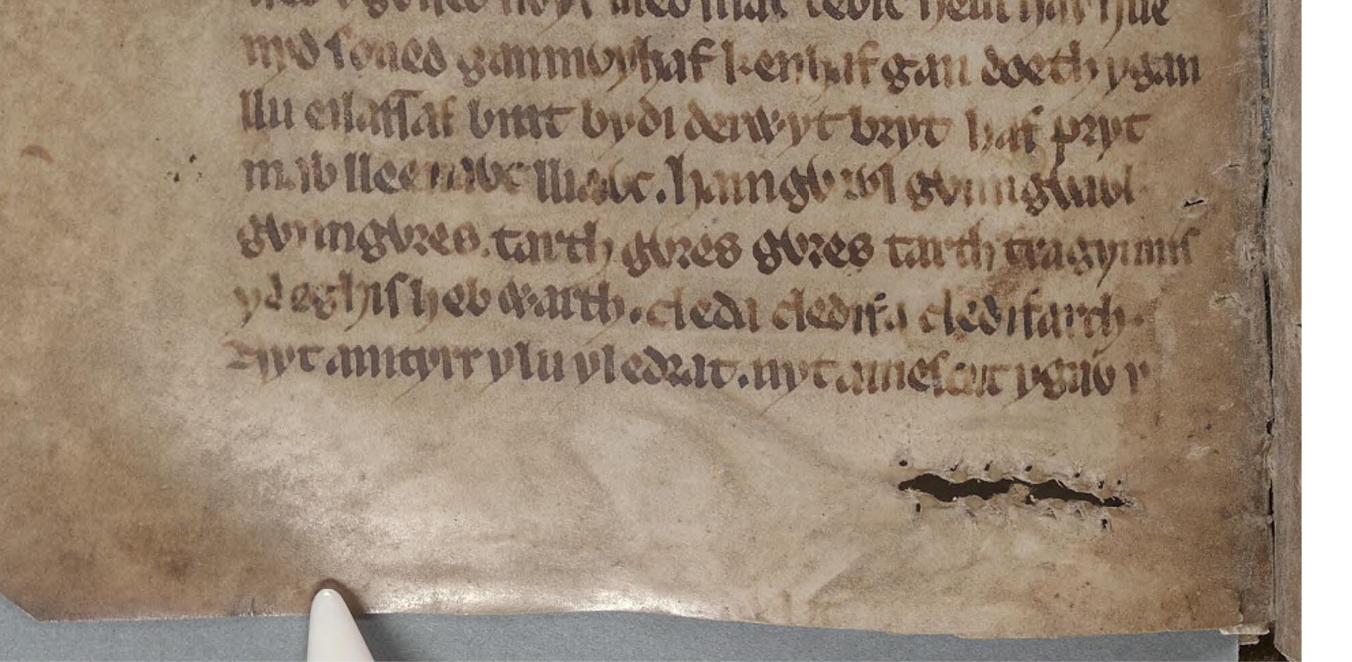
\includegraphics[width=\textwidth]{3orth/images/canvas.png}
    \caption[The bottom of \gls{bt} p.~64]{The bottom of \gls{bt} p.~64. Image credit: The National Library of Wales}
    \label{fig:p64}
\end{figure}

The easiest way to account for this situation is that scribe X86  copied the word \mw{kywlat} twice: first he wrote it as a catchword to make sure the quire starting with page 65 would be placed immediately following the quire ending with page 64. The second time it is found as the first word of page 65. In the first instance, he adds orthographic representation of lenition, and in the second he copies his exemplar directly. The reason he did not add lenition in the second instance is most likely due to him forgetting about the syntactic context of this word by the time he had his next quire before him. This instance singularly tells us that it was scribe X86 was the one who added orthographic lenition to his texts, and that his exemplar did not have lenition represented orthographically. 

\begin{mylongtable}{@{}lrrrlllll@{}}
\toprule
\textbf{IW} & \textbf{L.} & \textbf{P.\ MS} & \textbf{L.\ MS} & \textbf{Word} & \textbf{Translation} & \textbf{Cause of lenition} & \textbf{Represented} & \textbf{Initial C} \\ \midrule\endhead
II & 1 & 56 & 14 & \mw{gan} & `with' & petr & yes & c \\
II & 2 & 56 & 14 & \mw{wledic} & `lord' & \mw{am} & yes & g \\
II & 2 & 56 & 15 & \mw{gỽarthegyd} & `cowherd' & prep adj & no & g \\
II & 4 & 56 & 16 & \mw{teyrned} & `kingship' & obj len? & no & t \\
II & 7 & 56 & 19 & \mw{kyuygyd} & `warrior' & \mw{prep noun} & no & c \\
II & 9 & 56 & 20 & \mw{oꝛmes} & `oppression' & \mw{dy} & yes & g \\
II & 10 & 56 & 21 & \mw{dꝛos} & `over' & petr & yes & t \\
II & 11 & 56 & 21 & \mw{wyr} & `men' & obj len? & yes & g \\
II & 13 & 56 & 23 & \mw{tỽrỽf} & `clamour' & obj len? & no & t \\
II & 17 & 56 & 26 & \mw{wyr} & `men' & obj len? & yes & g \\
II & 19 & 57 & 1 & \mw{tanc} & `peace' & obj len? & no & t \\
II & 19 & 57 & 1 & \mw{gan} & `with' & petr & yes & c \\
II & 21 & 57 & 3 & \mw{gynrein} & `princes' & \mw{y} `his' & yes & c \\
II & 21 & 57 & 3 & \mw{kyỽym don} & `??' & ?? & no & c \\
II & 23 & 57 & 4 & \mw{wyr} & `men' & obj len? & yes & g \\
II & 24 & 57 & 5 & \mw{uaglei} & `snared' & \mw{a} & yes & m \\
II & 25 & 57 & 6 & \mw{kat} & `battle' & \mw{ỽrth} & no & c \\
II & 26 & 57 & 7 & \mw{pỽyllatt} & `knew' & \mw{pan} & no & p \\
II & 27 & 57 & 7 & \mw{ueidat} & `dared' & \mw{pan} & yes & b \\
II & 29 & 57 & 9 & \mw{alon} & `enemies' & \mw{e} `his' & yes & g \\
II & 29 & 57 & 9 & \mw{wen} & `white' & feminine noun & yes & g \\
II & 33 & 57 & 11 & \mw{vallỽyf} & `die' & \mw{yny} & yes & b \\
III & 6 & 57 & 16 & \mw{weſceryd} & `scatters' & \mw{yt} & yes & g \\
III & 8 & 57 & 16 & \mw{vo} & `may be' & \mw{tra} & yes & b \\
III & 8 & 57 & 16--17 & \mw{uuch/yd} & `life' & \mw{dy} & yes & b \\
III & 10 & 57 & 17 & \mw{gan} & `with' & petr & yes & c \\
III & 10 & 57 & 17 & \mw{clotuan} & `famous man' & \mw{gan} & no & c \\
III & 12 & 57 & 18 & \mw{vot} & `that … is' & ?? & yes & b \\
III & 12 & 57 & 18 & \mw{plant} & `children' & \mw{e} `his' & no & p \\
III & 14 & 57 & 19 & \mw{oꝛuchel} & `very high' & \mw{yn} & yes & g \\
III & 14 & 57 & 19 & \mw{wledic} & `lord' & prep adj & yes & g \\
III & 16 & 57 & 29 & \mw{keimyat} & `champion' & \mw{yn} & no & c \\
III & 19 & 57 & 21 & \mw{gaỽſſant} & `received' & \mw{a} & yes & c \\
III & 20 & 57 & 22 & \mw{godyant} & `rose' & parenthesis & yes & c \\
III & 23 & 57 & 23 & \mw{collet} & `lost' & prep adj & no & c \\
III & 25 & 57 & 23--24 & \mw{gaf/fel} & `have' & \mw{heb} & yes & c \\
III & 30 & 57 & 25 & \mw{pop} & `every' & \mw{o} & no & p \\
III & 31 & 57 & 26 & \mw{peleitrat} & `spear blow' & \mw{dy} & no & p \\
III & 32 & 57 & 26 & \mw{kat} & `battle' & verb ending? & no & c \\
III & 34 & 58 & 1 & \mw{wneit} & `you do' & \mw{a} & yes & g \\
III & 39 & 58 & 4 & \mw{waeſſaf} & `pledge' & \mw{heb} & yes & g \\
III & 40 & 58 & 4 & \mw{teyrn} & `ruler' & \mw{am} & no & t \\
III & 43 & 58 & 5 & \mw{uu} & `was' & \mw{a} & yes & b \\
III & 43 & 58 & 5 & \mw{uyd} & `will be' & \mw{a} & yes & b \\
III & 44 & 58 & 6 & \mw{kyſtedlyd} & `fellow' & \mw{oes} & no & c \\
III & 45 & 58 & 6 & \mw{dꝛemher} & `is seen' & \mw{pan} & yes & t \\
III & 48 & 58 & 8 & \mw{teyrn} & `ruler' & \mw{am} & no & t \\
III & 53 & 58 & 10 & \mw{vallỽyf} & `die' & \mw{yny} & yes & b \\
IV & 3 & 58 & 13 & \mw{parch} & `praise' & obj len? & no & p \\
IV & 6 & 58 & 15 & \mw{oꝛuoled} & `jubilation' & \mw{y} `to' & yes & g \\
IV & 7 & 58 & 15 & \mw{tired} & `lands' & prep adj & no & t \\
IV & 17 & 58 & 18 & \mw{lad} & `kills' & \mw{yt} & yes & ll \\
IV & 17 & 58 & 18 & \mw{gryc} & `hangs' & \mw{yt} & yes & c \\
IV & 18 & 58 & 19 & \mw{vac} & `cherishes' & \mw{yt} & yes & m \\
IV & 18 & 58 & 19 & \mw{vyc} & `honours' & \mw{yt} & yes & m \\
IV & 19 & 58 & 19 & \mw{vyc} & `honours' & \mw{yt} & yes & m \\
IV & 19 & 58 & 19 & \mw{vac} & `cherishes' & \mw{yt} & yes & m \\
IV & 20 & 58 & 19 & \mw{lad} & `kills' & \mw{yt} & yes & ll \\
IV & 22 & 58 & 20 & \mw{veird} & `bards' & \mw{y} `to' & yes & b \\
IV & 23 & 58 & 20 & \mw{geugant} & `certain' & \mw{yn } & yes & c \\
IV & 24 & 58 & 21 & \mw{wedant} & `they say' & \mw{yt} & yes & g \\
IV & 26 & 58 & 21--22 & \mw{pe/riſ} & `caused' & \mw{th} & no & p \\
IV & 35 & 58 & 25 & \mw{tỽrỽf} & `tumult' & prep adj & no & t \\
IV & 38 & 58 & 26 & \mw{trefret} & `homestead' & prep adj & no & t \\
IV & 39 & 58 & 26 & \mw{tudet} & `clothing' & prep adj & no & t \\
IV & 41 & 59 & 1 & \mw{van} & `bright' & epithet & yes & m \\
IV & 43 & 59 & 1 & \mw{trygan} & `sound' & \mw{un} & no & t \\
IV & 45 & 59 & 2 & \mw{gan} & `with' & epithet & yes & c \\
IV & 48 & 59 & 3 & \mw{gigleu} & `heard' & \mw{a} & yes & c \\
IV & 49 & 59 & 3 & \mw{ỽrdlideu} & `attributes' & \mw{y} `to' & yes & g \\
IV & 51 & 59 & 4 & \mw{weithredeu} & `works' & \mw{dy} & yes & g \\
IV & 52 & 59 & 4 & \mw{vallỽyf} & `die' & \mw{yny} & yes & b \\
V & 1 & 59 & 7 & \mw{blyned} & `years' & \mw{un} & no & b \\
V & 6 & 59 & 9 & \mw{vereu} & `spit' & \mw{am} & yes & b \\
V & 8 & 59 & 9--10 & \mw{gỽydua/eu} & `seats' & prep adj & no & c \\
V & 9 & 59 & 10 & \mw{wyt} & `food' & \mw{e} `his' & yes & b \\
V & 11 & 59 & 11 & \mw{varch} & `horse' & \mw{e} `his' & yes & m \\
V & 11 & 59 & 11 & \mw{danaỽ} & `under him' & petr & yes & t \\
V & 16 & 59 & 13 & \mw{loi} & `calves' & \mw{o} & yes & ll \\
V & 20 & 59 & 14 & \mw{lleas} & `death' & \mw{bei} & no & ll \\
V & 22 & 59 & 15 & \mw{kygryn} & `shivering' & feminine noun & no & c \\
V & 22 & 59 & 15 & \mw{kygryt} & `trembling' & feminine noun & no & c \\
V & 23 & 59 & 15 & \mw{wen} & `white' & feminine noun & yes & g \\
V & 23 & 59 & 15--16 & \mw{olch/et} & `washed' & feminine noun & yes & g \\
V & 26 & 59 & 26 & \mw{waet} & `blood' & \mw{am} & yes & g \\
V & 28 & 59 & 17 & \mw{uei} & `would be' & \mw{a} & yes & b \\
V & 28 & 59 & 17 & \mw{wedỽ} & `widow' & \mw{uei} & yes & g \\
V & 28 & 59 & 17 & \mw{wreic} & `wife' & \mw{y} `his' & yes & g \\
V & 30 & 59 & 18 & \mw{mynyc} & `frequent' & prep adj & no & m \\
V & 31 & 59 & 19 & \mw{poꝛth} & `gate' & \mw{am} & no & p \\
V & 31 & 59 & 19 & \mw{pen} & `head' & \mw{am} & no & p \\
V & 34 & 59 & 21 & \mw{trỽſt} & `noise' & \mw{py} & no & t \\
V & 35 & 59 & 21 & \mw{gryn} & `swells' & \mw{a} & yes & c \\
V & 38 & 59 & 22 & \mw{pedyt} & `infantry' & \mw{y} `his' & no & p \\
V & 44 & 59 & 25 & \mw{orꝛuyd} & `conquers' & \mw{a} & yes & g \\
V & 48 & 60 & 1 & \mw{blaỽd} & `strikes' & \mw{a} & yes & p \\
V & 54 & 60 & 3 & \mw{gylchyn} & `surroundings' & \mw{y} `his' & yes & c \\
V & 56 & 60 & 4 & \mw{par} & `spear' & \mw{y} `his' & no & p \\
V & 58 & 60 & 5 & \mw{vallỽyf} & `die' & \mw{yny} & yes & b \\
VI & 1 & 60 & 8 & \mw{uaỽr} & `big' & feminine noun & yes & m \\
VI & 1 & 60 & 8 & \mw{uu} & `was' & \mw{a} & yes & b \\
VI & 2 & 60 & 9 & \mw{gynnu} & `descends' & \mw{pan} & yes & c \\
VI & 7 & 60 & 12 & \mw{vaỽr} & `big' & epithet & yes & m \\
VI & 7 & 60 & 13 & \mw{trebyſtaỽt} & `commotion' & prep adj & no & t \\
VI & 8 & 60 & 13 & \mw{paraỽt} & `ready' & NP lenition & no & p \\
VI & 10 & 60 & 15 & \mw{paraỽt} & `ready' & NP lenition & no & p \\
VI & 11 & 60 & 15 & \mw{vab} & `son' & epithet & yes & m \\
VI & 11 & 60 & 16 & \mw{kymỽyaỽc} & `grieving' & \mw{-ei} & no & c \\
VI & 12 & 60 & 16 & \mw{leỽ} & `valiant' & prep adj & yes & g \\
VI & 12 & 60 & 16 & \mw{ỽyſtyl} & `bledge' & \mw{o} & yes & g \\
VI & 14 & 60 & 18 & \mw{gerenhyd} & `kindred' & \mw{am} & yes & c \\
VI & 17 & 60 & 20 & \mw{peleidyr} & `spears' & obj len? & no & p \\
VI & 18 & 60 & 21 & \mw{luyd} & `hosts' & \mw{y} `his' & yes & ll \\
VI & 19 & 60 & 21 & \mw{gyweithyd} & `company' & \mw{e} `his' & yes & c \\
VI & 22 & 60 & 23 & \mw{vꝛein} & `crows' & \mw{-ei} & yes & b \\
VI & 23 & 60 & 23 & \mw{gr\.{y}ſſỽys} & `charged' & \mw{a} & yes & c \\
VI & 23 & 60 & 24 & \mw{gan} & `with' & petr & yes & c \\
VI & 24 & 60 & 24 & \mw{blỽydyn} & `year' & obj len?/adv? & no & b \\
VI & 25 & 60 & 25 & \mw{vallỽyf} & `die' & \mw{yny} & yes & b \\
XI & 2 & 29 & 22 & \mw{biewyd} & `will have' & [\mw{a}] & yes & p \\
XI & 2 & 29 & 22 & \mw{gyneiluoaỽc} & `supporter' & \mw{obj len?} & yes & c \\
XI & 7 & 29 & 25 & \mw{bꝛydein} & (place name) & \mw{o} & yes & p \\
XI & 7 & 29 & 26 & \mw{gofein} & `memories' & \mw{prep noun} & yes & c \\
XI & 8 & 29 & 26 & \mw{berth} & `bush' & \mw{o} & yes & p \\
XI & 9 & 29--30 & 26--1 & \mw{ky/uerbyn} & `opposition' & \mw{obj len} & no & c \\
XI & 11 & 30 & 2 & \mw{lyghes} & `fleet' & \mw{y} `to' & yes & ll \\
XI & 12 & 30 & 2 & \mw{beleidyr} & `lances' & \mw{o} & yes & p \\
XI & 12 & 30 & 2 & \mw{bleigheit} & `battle' & \mw{o} & yes & p \\
XI & 12 & 30 & 2--3 & \mw{pꝛen/wres} & `??' & \mw{??} & ?? & ?? \\
XI & 13 & 30 & 3 & \mw{paỽb} & `everyone' & \mw{y} `to' & no & p \\
XI & 13 & 30 & 3 & \mw{trachwres} & `fury' & \mw{y} `his' & no & t \\
XI & 14 & 30 & 4 & \mw{gadeu} & `battles' & \mw{o} & yes & c \\
XI & 18 & 30 & 6 & \mw{vꝛetrỽyn} & (place name) & feminine noun & yes & b \\
XI & 18 & 30 & 7 & \mw{wres} & `heat' & \mw{trỽy} & yes & g \\
XI & 18 & 30 & 7 & \mw{tan} & `fire' & prep adj & no & t \\
XI & 19 & 30 & 7 & \mw{trachwres} & `fury' & \mw{y} `his' & no & t \\
XI & 23 & 30 & 10 & \mw{veibon} & `sons' & \mw{y} `to' & yes & m \\
XI & 25 & 30 & 11 & \mw{alon} & `enemies' & \mw{dy} & yes & g \\
XI & 27 & 30 & 11 & \mw{uraỽt} & `judgment' & \mw{ad} & yes & b \\
XI & 30 & 30 & 14 & \mw{gan} & `with' & petr & yes & c \\
XI & 30 & 30 & 14 & \mw{waỽꝛ} & `dawn' & \mw{gan} & yes & g \\
XI & 37 & 30 & 18 & \mw{wnaỽ} & `may do' & \mw{a} & yes & g \\
XI & 43 & 30 & 22 & \mw{gaenaỽc} & `armoured' & prep adj & yes & c \\
XI & 44 & 30 & 22 & \mw{wyl} & `sees' & \mw{ny} & yes & g \\
XI & 44 & 30 & 22 & \mw{welas} & `saw' & \mw{ny} & yes & g \\
XII & 1 & 63 & 25 & \mw{goꝛchoꝛdyon} & `hosts' & parenthesis & no & g \\
XII & 3 & 64 & 1 & \mw{gogyfres} & `united assault' & \mw{obj len} & no & g \\
XII & 5 & 64 & 2 & \mw{golychaf} & `I praise' & \mw{ny/[ry]} & no & g \\
XII & 5 & 64 & 2 & \mw{g(n)awd} & `praise' & \mw{a[r]} & no & g \\
XII & 5 & 64 & 2 & \mw{vꝛython} & (place name) & \mw{o} & yes & b \\
XII & 8 & 64 & 4 & \mw{wledic} & `ruler' & \mw{y} `to' & yes & g \\
XII & 9 & 64 & 5 & \mw{wlat} & `country' & fem art & yes & g \\
XII & 12 & 64 & 7 & \mw{wledic} & `ruler' & \mw{y} `to' & yes & g \\
XII & 12 & 64 & 7 & \mw{omed} & `refuses' & \mw{ni} & yes & g \\
XII & 14 & 64 & 8 & \mw{vyỽ} & `life' & \mw{y} `his' & yes & b \\
XII & 17 & 64 & 10 & \mw{pꝛeſſennaỽl} & `present' & fem noun & no & p \\
XII & 18 & 64 & 11 & \mw{gohoyỽ} & `fine' & \mw{ry} & no & g \\
XII & 18 & 64 & 11 & \mw{lyccraỽꝛ} & `is corrupted' & \mw{ry} & yes & ll \\
XII & 18 & 64 & 11 & \mw{lyccrer} & `must be corrupted' & \mw{ry} & yes & ll \\
XII & 19 & 64 & 12 & \mw{barnaỽꝛ} & `is judged' & \mw{ry} & no & b \\
XII & 20 & 64 & 12 & \mw{barn} & `judges' & \mw{ry} & no & b \\
XII & 22 & 64 & 13 & \mw{gỽr} & `man' & \mw{y} `to' & no & g \\
XII & 23 & 64 & 14 & \mw{traet} & `feet' & \mw{go} & no & t \\
XII & 25 & 64 & 15 & \mw{tebet} & `retreat' & \mw{ar} & no & t \\
XII & 26 & 64 & 16 & \mw{ofyn} & `ask' & \mw{ny} & yes & g \\
XII & 26 & 64 & 16 & \mw{wnech} & `may do' & \mw{a} & yes & g \\
XII & 30 & 64 & 18 & \mw{gynan} & (personal name) & parenthesis & yes & c \\
XII & 35 & 64 & 21 & \mw{gan} & `song' & prep noun & yes & c \\
XII & 36 & 64 & 21 & \mw{gan} & `with' & petr & yes & c \\
XII & 36 & 64 & 21 & \mw{gan} & `with' & petr & yes & c \\
XII & 36 & 64 & 22 & \mw{llu} & `host' & \mw{gan} & no & ll \\
XII & 37 & 64 & 22 & \mw{bydi} & `??' & NP lenition & yes & p \\
XII & 37 & 64 & 22 & \mw{bꝛyt} & `??' & \mw{??} & yes & p \\
XII & 38 & 64 & 23 & \mw{gỽaỽl} & (personal name) & \mw{ham} & no & g \\
XII & 39 & 64 & 24 & \mw{gỽres} & `heat' & obj len? & no & g \\
XII & 40 & 64 & 24 & \mw{gynniſ} & `kindled' & \mw{tra} & yes & c \\
XII & 42 & 64 & 26 & \mw{lu} & `host' & \mw{y} `his' & yes & ll \\
XII & 42 & 64 & 26 & \mw{ledꝛat} & `stealth' & \mw{y} `to' & yes & ll \\
XII & 43 & 64 & 26 & \mw{gaỽ} & `stop' & \mw{y} `to' & yes & c \\
XII & 43 & 64 & 27 & \mw{gywlat} & `enemy' & \mw{y} `his' & yes & c \\
XII & 44 & 65 & 1 & \mw{veirch} & `horses' & \mw{y} `his' & yes & m \\
XII & 45 & 65 & 2 & \mw{march} & `horse' & \mw{o} & no & m \\
XII & 46 & 65 & 2 & \mw{car} & `loves' & \mw{th} & no & c \\
XII & 48 & 65 & 3 & \mw{gaer} & (place name) & \mw{o} & yes & c \\
XII & 48 & 65 & 3 & \mw{glut} & (place name) & fem noun & yes & c \\
XII & 48 & 65 & 3--4 & \mw{ga/er} & (place name) & \mw{hyt} & yes & c \\
XII & 48 & 65 & 4 & \mw{garadaỽc} & (place name) & fem noun & yes & c \\
XII & 49 & 65 & 4 & \mw{gỽallaỽc} & (personal name) & \mw{a} & no & g \\ \bottomrule
\caption{CT}
\label{my-label}
\end{mylongtable}

\subsection{Armes Prydein Vawr}
The poem \mw{Armes Prydein Vawr} `the Great Prophecy of Britain' is also found in the \gls{bt} on pages 13--18. It is independently dateable on the basis of the political elements found in it. Ifor Williams argues that the poem was composed before the Norman conquest of 1066, because it prophecies deliverance from the Saxons, and there is no point in making such a prophecy when the result of this would be that the Normans would still be in power. Furthermore, the poem differentiates between men of Dublin and Irishmen of Ireland, meaning the poem postdates the settlement of the Vikings in the ninth century. In addition, the name \mw{Glywysing} is used for an area roughly coterminous with Glamorgan, which Williams considers an archaism. Ifor Williams dates the composition of this poem to about 900 on the basis of these considerations~\autocite[x--xii]{williams_armes_1955}. \Textcite{dumville_brittany_1983} dates the poem to a date later in the tenth century. 


\begin{table}[h]
\centering
\begin{tabular}{@{}rlll@{}}
\toprule
 & \textbf{Rep.} & \textbf{Not rep.} & \textbf{Total} \\ \midrule
T & 62 & 25 & 87 \\
Not T & 55 & 8 & 63 \\
\textbf{Total} & \textbf{117} & \textbf{33} & \textbf{150} \\ \bottomrule
\end{tabular}
\caption{Correspondence between initial consonant type and orthographic representation of lenition in \mw{Armes Prydein Vawr}.}
\label{armesprydeinnumbers}
\end{table}

% Table \ref{armesprydeinnumbers} shows that there is a correlation between consonant type and lenition. The two-tailed P value according to Fisher's exact test equals $0.0272<0.05$. This shows that the null hypothesis (the initial consonant being a voiceless stop or another consonant has no bearing upon orthographic representation of lenition) must be rejected.

It is the distribution, not the raw frequency of non-orthographical representation that tells us about the date of an exemplar. Nevertheless, only a minority of about two-fifths of the voiceless stops are not lenited. This number agrees with the other prophecies.

\subsubsection{Hypercorrect insertion of lenition}
In several cases, lenition is written where I have no explanation for it. They are found in the following lines (translations taken from \textcite{williams_armes_1972}):

\begin{mwl}
\mwc[gwssyl]{\mw{Armes Prydein} l.~108 (\gls{bt} 16.7)}{pan dyffo iwyſ y vn gỽſſyl}{when the men of Wessex will come together in council,}
\mwc[gyghor]{\mw{Armes Prydein} l.~109 (\gls{bt} 16.7--8}{Vn coꝛ vn gyg/hoꝛ a lloegyr lloscit}{in a single party, of one mind with the Mercian incendiaries,}
\end{mwl}

Both examples contain a lenited masculine noun after \mw{vn} `one'. 
Example~\ref{gwssyl} has \mw[council]{gỽſſyl}, and  Example~\ref{gyghor} has \mw[council]{gyghoꝛ}. 
Two words that mean roughly the same are erroneously lenited under the same circumstances, and they are on the same line in the manuscript. In the second case, (non-represented) lenition of \mw{coꝛ} `party' may have influenced the decision to write lenition here\footnote{\mw{coꝛ} `party' is itself problematic here. \Textcite[s.v.\ côr\textsuperscript{1}]{bevan_geiriadur_2014} shows that this word may be both masculine and feminine, but l~48 \mw{goꝛ}	`meeting' may imply that it was feminine at least in this instance.}. Another possible solution is that \mw{un} means not `one', but `same' in both problematic instances. If this is the case, then lenition is justified, as \mw{un} meaning `same' may be considered a preposed adjective. Even if this is not what the author of the original composition meant to say, it is possible that the scribe of the \gls{bt} understood \mw{un} as such here, and lenited accordingly.



\subsubsection{Non-representation of lenition of ¬\acrshort{T}}
Among the non-voiceless stops whose lenition is not represented orthographically, all cases except one have an initial \mw{g}. Perhaps this is a relic from the \gls{ow} practice to represent /\cw/ with \mw{gu}. Etymologically, each of these cases except one has a /\cw/ following the /g/: l.~8	\mw{goꝛuoled},
l.~58	\mw{Gỽy},
l.~123	\mw{gỽerth},
l.~143	\mw{gỽerth},
l.~151	\mw{gỽyr}, and
l.~167	\mw{gỽlatwarthegyd}, while
l.~176	\mw{gynhon} starts with an etymological /g/. 

The one remaining case is l.~80	\mw{mỽyn} `benefit', which should be lenited due to parenthesis in the following line: 
\mwcc[mwyn]{\mw{Armes Prydein} l.~80 (\gls{bt} 15.11--12)}{ny byd y vedyc mỽyn oꝛ a wnaant.}{The doctor will not have benefit from what they do.}
Here, \mw[benefit]{mỽyn} follows the noun \mw[doctor]{vedyc} and may therefore have been misinterpreted by the scribe as adjective \mw[mild, tender]{mwyn}. 
Regardless of the validity of this explanation, this assumes that lenition of a non-voiceless stop was not represented in an original composition either. 
This means that this word presents a singular counterexample to the argument that \mw{Armes Prydein} stems from a period when lenition was written, but not lenition of voiceless stops.



\begin{mylongtable}{@{}rlllll@{}}
\toprule
\textbf{Line} & \textbf{Word} & \textbf{Translation} & \textbf{Cause of lenition} & \textbf{Represented} \\ \midrule\endhead
2 & \mw{genhyn} & `with them' & petrified lenition & yes \\
7 & \mw{Gaer} & `Fort' & \mw{hyt} & yes \\
7 & \mw{Weir} & (place name) & feminine noun & yes \\
8 & \mw{goꝛuoled} & `jubilation' & object lenition & no \\
11 & \mw{genhyn} & `with them' & petrified lenition & yes \\
12 & \mw{uyd} & `will be' & [\mw{a}] & yes \\
19 & \mw{gỽynyn} & `they complain' & \mw{a} & yes \\
22 & \mw{telhyn} & `they pay' & \mw{a} & no \\
23 & \mw{ỽr} & `man' & NP lenition & yes \\
24 & \mw{talei} & `will pay' & \mw{a} & no \\
25 & \mw{eir} & `word' & \mw{a} `from' & yes \\
30 & \mw{wydynt} & `they know' & \mw{ny} & yes \\
30 & \mw{treiglynt} & `they pass' & \mw{py} & no \\
31 & \mw{pꝛynaſſant} & `they bought' & \mw{pan} & no \\
31 & \mw{Danet} & (place name) & object lenition & yes \\
32 & \mw{gan} & `by' & petrified lenition & yes \\
35 & \mw{wiraỽt} & `liquor' & preposed adjective & yes \\
35 & \mw{ved} & `mead' & \mw{o} & yes \\
40 & \mw{uyd} & `will be' & \mw{pan} & yes \\
41 & \mw{bỽyller} & `is intended' & \mw{a} & yes \\
42 & \mw{Vꝛython} & `Britons' & feminine noun & yes \\
45 & \mw{eir} & `word' & \mw{a} `from' & yes \\
48 & \mw{goꝛ} & `meeting' & \mw{un} & yes \\
48 & \mw{gyghoꝛ} & `council' & \mw{un} & yes \\
55 & \mw{lan} & `edge' & \mw{am} & yes \\
56 & \mw{vydinaỽr} & `armies' & preposed adjective & yes \\
58 & \mw{Gỽy} & (place name) & \mw{am} & no \\
58 & \mw{peurllyn} & `bright lake' & \mw{am} & no \\
61 & \mw{kynyrcheit} & `gathering' & preposed genitive & no \\
62 & \mw{von} & `stem' & \mw{ỽrth} & yes \\
65 & \mw{goet} & `wood' & \mw{trỽy} & yes \\
66 & \mw{uỽꝛch} & `wall' & \mw{trỽy} & yes \\
67 & \mw{tir} & `land' & \mw{y} `to' & no \\
68 & \mw{laỽ} & `hand' & \mw{trỽy} & yes \\
68 & \mw{gyghoꝛ} & `council' & feminine noun & yes \\
69 & \mw{Geri} & (place name) & feminine noun & yes \\
74 & \mw{watwar} & `taunting' & preposed adjective & yes \\
76 & \mw{oꝛolchant} & `drench' & \mw{a} & yes \\
77 & \mw{kyneircheit} & `courtiers' & preposed genitive & no \\
80 & \mw{vedyc} & `doctor' & \mw{y} `to' & yes \\
80 & \mw{mỽyn} & `benefit' & parenthesis & no \\
80 & \mw{wnaant} & `they do' & \mw{a} & yes \\
82 & \mw{wnant} & `they do' & \mw{a} & yes \\
84 & \mw{ỽdant} & `they know' & \mw{a} & yes \\
88 & \mw{gerd} & `goes' & \mw{a} & yes \\
88 & \mw{genhyn} & `with them' & petrified lenition & yes \\
91 & \mw{baladyr} & `lance' & \mw{yn} & yes \\
91 & \mw{gan} & `with' & petrified lenition & yes \\
93 & \mw{dꝛoſ} & `over' & petrified lenition & yes \\
94 & \mw{rud} & `cheek' & \mw{ar} & yes \\
96 & \mw{Gaer} & `Fort' & \mw{hyt} & yes \\
96 & \mw{Wynt} & (place name) & feminine noun & yes \\
97 & \mw{Gymry} & `Welshmen' & epithet & yes \\
98 & \mw{trindaỽt} & `trinity' & feminine article & no \\
98 & \mw{gynt} & `former' & adverbial phrase & yes \\
102 & \mw{genhyn} & `with them' & petrified lenition & yes \\
103 & \mw{talet} & `payment' & \mw{heb} & no \\
103 & \mw{dynget} & `fate' & \mw{o} & yes \\
103 & \mw{geffyn} & `we have' & \mw{a} & yes \\
104 & \mw{veibon} & `sons' & preposed adjective & yes \\
108 & \mw{gỽſſyl} & `council' & ?? & yes \\
109 & \mw{gyghoꝛ} & `council' & ?? & yes \\
110 & \mw{luyd} & `host' & preposed adjective & yes \\
111 & \mw{beunyd} & `every day' & adverbial phrase & yes \\
112 & \mw{ỽyr} & `knows' & \mw{ny} & yes \\
112 & \mw{uyd} & `will be' & [\mw{a}] & yes \\
113 & \mw{gyfarth} & `barking' & object lenition & yes \\
113 & \mw{vynyd} & `mountain' & \mw{o} & yes \\
114 & \mw{talu} & `pay' & \mw{\.{y}} `to' & no \\
116 & \mw{coꝛff} & `body' & object lenition & no \\
116 & \mw{gilyd} & `companion' & \mw{y} `his' & yes \\
122 & \mw{galaned} & `corpses' & subject of plural verb & yes \\
123 & \mw{treth} & `tax' & feminine article & no \\
123 & \mw{gỽerth} & `value' & \mw{ar} & no \\
123 & \mw{beunyd} & `every day' & adverbial phrase & yes \\
124 & \mw{gennadeu} & `messengers' & preposed adjective & yes \\
124 & \mw{luyd} & `host' & preposed adjective & yes \\
125 & \mw{kyfergyr} & `conflict' & \mw{trỽy} & no \\
126 & \mw{gyweir} & `ordered' & \mw{yn} & yes \\
126 & \mw{gyteir} & `unanimous' & adverbial phrase & yes \\
126 & \mw{g\.{y}tſon} & `harmonious' & adverbial phrase & yes \\
126 & \mw{gytffyd} & `of one faith' & adverbial phrase & yes \\
127 & \mw{peri} & `cause' & \mw{y} `to' & no \\
128 & \mw{gynnullant} & `they assemble' & \mw{a} & yes \\
130 & \mw{tywyſſaỽ} & `lead' & \mw{y} `to' & no \\
130 & \mw{lieingant} & `circle of linen' & \mw{trỽy} & yes \\
131 & \mw{genhyn} & `with them' & petrified lenition & yes \\
132 & \mw{gat} & `battle' & feminine article & yes \\
133 & \mw{geiſſyſſant} & `they seek' & [\mw{a}] & yes \\
134 & \mw{wlad} & `country' & feminine article & yes \\
136 & \mw{vꝛo} & `land' & \mw{py} & yes \\
137 & \mw{genhyn} & `with them' & petrified lenition & yes \\
138 & \mw{wir} & `true' & \mw{o} & yes \\
139 & \mw{vꝛeint} & `privilage' & \mw{Neu} & yes \\
141 & \mw{Gymry} & `Welshmen' & subject of plural verb & yes \\
143 & \mw{talhont} & `they pay' & \mw{pan} & no \\
143 & \mw{gỽerth} & `worth' & preposed adjective & no \\
145 & \mw{garant} & `they love' & [\mw{a}] & yes \\
149 & \mw{lygheſ} & `fleet' & parenthesis & yes \\
150 & \mw{gat} & `battle' & feminine article & yes \\
151 & \mw{gỽyr} & `men' & parenthesis & no \\
152 & \mw{Pꝛydein} & `Britain' & \mw{o} & no \\
152 & \mw{virein} & `fair' & parenthesis & yes \\
152 & \mw{luyd} & `host' & preposed adjective & yes \\
153 & \mw{Lydaỽ} & `Brittany' & \mw{o} & yes \\
153 & \mw{pꝛydaỽ} & `lovely' & parenthesis & no \\
153 & \mw{gywiethyd} & `company' & preposed adjective & yes \\
154 & \mw{katueirch} & `warhorse' & \mw{ar} & no \\
155 & \mw{pop} & `every' & \mw{o} & no \\
157 & \mw{gyweithyd} & `company' & preposed adjective & yes \\
164 & \mw{vꝛaỽt} & `judgment' & \mw{hyt} & yes \\
166 & \mw{oꝛſegyn} & `trampler' & \mw{deu} & yes \\
166 & \mw{pleit} & `side' & \mw{o} & no \\
167 & \mw{gedaỽl} & `generous' & \mw{deu} & yes \\
167 & \mw{gỽlatwarthegyd} & `land-cowman' & preposed adjective & no \\
168 & \mw{baraỽt} & `ready' & preposed adjective & yes \\
169 & \mw{luyd} & `host' & preposed adjective & yes \\
170 & \mw{beunyd} & `every day' & adverbial phrase & yes \\
172 & \mw{Vynaỽ} & `Isle of Man' & \mw{o} & yes \\
172 & \mw{Lydaỽ} & `Brittany' & \mw{hyt} & yes \\
172 & \mw{vyd} & `will be' & \mw{yt} & yes \\
173 & \mw{Danet} & (place name) & \mw{hyt} & yes \\
173 & \mw{bieiuyd} & `will posess' & [\mw{a}] & yes \\
174 & \mw{Waỽl} & (place name) & \mw{o} & yes \\
174 & \mw{Weryt} & (place name) & \mw{hyt} & yes \\
176 & \mw{gynhon} & `tribes' & \mw{ar} & no \\
177 & \mw{Ỽydyl} & `Irishmen' & subject of plural verb & yes \\
178 & \mw{Gymry} & `Welshmen' & subject of plural verb & yes \\
178 & \mw{kadyr} & `powerful' & object lenition & no \\
178 & \mw{gyweithyd} & `company' & preposed adjective & yes \\
179 & \mw{gỽꝛỽf} & `ale' & \mw{am} & yes \\
180 & \mw{gedỽyſ} & `kept' & \mw{ry} & yes \\
181 & \mw{pop} & `every' & \mw{y} `to' & no \\
182 & \mw{gan} & `with' & petrified lenition & yes \\
182 & \mw{gilyd} & `companion' & \mw{y} `his' & yes \\
183 & \mw{alwaỽꝛ} & `call' & \mw{ny} & yes \\
183 & \mw{gynifwyr} & `warrior' & \mw{yn} & yes \\
184 & \mw{gyfnewitwyr} & `merchants' & \mw{e} `his' & yes \\
185 & \mw{uyd} & `will be' & [\mw{a}] & yes \\
186 & \mw{gymỽyeit} & `warriors' & feminine noun & yes \\
187 & \mw{galaned} & `corpses' & subject of plural verb & yes \\
188 & \mw{vyd} & `will be' & [\mw{a}] & yes \\
189 & \mw{gychwyn} & `start' & \mw{ar} & yes \\
191 & \mw{voꝛ} & `sea' & \mw{ar} & yes \\
191 & \mw{peunyd} & `every day' & petrified lenition & no \\
192 & \mw{vꝛaỽt} & `judgment' & \mw{hyt} & yes \\
193 & \mw{lyfraỽꝛ} & `books' & object lenition & yes \\
193 & \mw{bꝛydyd} & `poet' & preposed adjective & yes \\
195 & \mw{greỽys} & `created' & \mw{a} & yes \\
197 & \mw{Kaer} & `fort' & feminine noun & no \\
199 & \mw{ỽyỽ} & `withered' & \mw{ny} & yes \\
199 & \mw{wellyc} & `neglected' & \mw{ny} & yes \\ \bottomrule
\caption{Representation of lenition in \mw{Armes Prydein}}
\label{armesprydein}
\end{mylongtable}


\subsection{Prophecies}
Here, I discuss several prophecies together in one section. I discuss these together because they are similar linguistically and in terms of content, and usually not long enough to make reliable inferences about them individually. I have analysed eight out of ten poems edited in `Prophecies from the Book of Taliesin' by \textcite{haycock_prophecies_2013}. I have not included \mw{Gwawt Lud y mawr} and \mw{Yn wir dymbi Romani kar}, because they are not easily dateable. Other poems are datable, and Haycock dates them with varying degrees of certainty to the tenth to the thirteenth century, as shown in Table \ref{proprep}. 
\begin{table}[h]
\centering
\begin{tabular}{@{}llddddl@{}}
  \toprule
  \tch{Text} & \tch{Table} & \tchh{T} & \tchh{Not T} & \tch{Date}\\
                              &  & \tch{rep.} & \tch{not rep.} & \tch{rep.} & \tch{not rep.} \\ \midrule
  \mw{Daronwy} & \ref{prop1} & 5 & 13 & 21 & 0  & 13c \\
  \mw{Glaswawt Taliessin} & \ref{prop2} & 9 & 3 & 11 & 0 & 10--13c\\
  \mw{Kychwedyl a’m dodyw…} & \ref{prop3} & 19 & 5 & 28 & 4 & 13c\\
  \mw{Dygogan awen} & \ref{prop4} & 2 & 3 & 11 & 1 & ll.\ 1--4: 10c\\
  \mw{Kein gyfedwch} & \ref{prop5} & 7 & 3 & 10 & 0 & 13c\\
  \mw{Rydyrchafwy Duw…} & \ref{prop6} & 6 & 5 & 15 & 1 & 10--13c\\
  \mw{Ymarwar Llud bychan} & \ref{prop9} & 1 & 4 & 5 & 1 & 10c\\
  \mw{Darogan Kadwal[adyr]} & \ref{prop10} & 5 & 2 & 3 & 0 & pre-Norman\\
  {Total} &  & {54} & {38} & {104} & {7} & \\ \bottomrule
\end{tabular}
\caption{Representation of lenition in the prophetic texts and their dates of composition according to \textcite[\emph{passim}]{haycock_prophecies_2013}.}
\label{proprep}
\end{table}

Table~\ref{proprep} shows that lenition of voiceless stops was not represented in about forty~per cent of cases. For other consonants, non-representation of lenition is confined to a handful of instances, which are best discussed individually.

Haycock's poems dated to the tenth until the thirteenth century have little positive evidence pointing towards a date in the later end of the spectrum. Typically, these poems have historical references pointing to the tenth century, but a date up to the thirteenth-century may not be excluded as long as there is no evidence to do so. Nevertheless, I will assume for the purpose of this chapter that these poems were written when they were most relevant, edging closer to a starting date. 

\subsubsection{Non-representation of lenition of ¬T}
Two out of seven non-represented lenited non-voiceless stops were expected to cause object lenition. Table~\ref{propobjlen} shows all instances where object lenition may be represented, but it is only represented twice. Both voiceless stops and other consonants are often left unlenited. \Textcite[72--73]{van_development14} shows that verbal endings causing object lenition initially did not cause object lenition. Rather, it has developed over the course of the \gls{mw} period. Before the thirteenth century, object lenition was not typically written, although object lenition may sometimes leak through in exemplars from the thirteenth century onward. I assume that the same is the case here: although the scribe of the \gls{bt} may have had object lenition as part of his Welsh grammar, the exemplars he copied most likely predated object lenition, and were thus inconsistently modernised in a manner similar to how the representation of lenited voiceless stops came to be modernised irregularly.

\begin{table}[h]
\centering
\begin{tabular}{@{}lllll@{}}
\toprule
\textbf{Poem} & \textbf{Line} & \textbf{Word} & \textbf{Translation} & \textbf{rep.} \\ \midrule
\mw{Daronwy} & 44 & \mw{kamualhau} & `hide' & no \\
\mw{Kychwedyl a’m dodyw…} & 13 & \mw{trỽy/det} & `passage' & no \\
\mw{Kychwedyl a’m dodyw…} & 18 & \mw{biỽ} & `cattle' & no \\
\mw{Dygogan awen} & 25 & \mw{kyfamrud} & `bloodshed' & no \\
\mw{Rydyrchafwy Duw…} & 10 & \mw{wyr} & `men' & yes \\
\mw{Ymarwar Llud bychan} & 3 & \mw{Pꝛydein} & (place name) & no \\
\mw{Ymarwar Llud bychan} & 18 & \mw{mab} & `son' & no \\
\mw{Darogan Kadwal[adyr]} & 15 & \mw{gelein} & `corpse' & yes \\ \bottomrule
\end{tabular}
\caption{Representation of object lenition in the Prophecies from the \gls{bt}}
\label{propobjlen}
\end{table}

A few instances of non-representation of lenition are found in Example~\ref{gwyargorgolchei}. 
\mwcc[gwyargorgolchei]{\mw{Kychwedyl} l.\ 53 (\gls{bt} 39.20--21)}{gỽyar goꝛgol/che[i] gỽarthaf iat.}{blood washed over the top of the head(s).}
Here, we would expect \mw{goꝛgolchei} `washed over' to be lenited, because it follows its subject and therefore is preceded by verbal particle \mw{a}, which may or may not be written out in full, but always causes lenition. Additionally, the ending in \ei\ consistently causes lenition throughout the \gls{mw} period, and therefore \mw{gỽarthafiat} `heads' should be lenited~\Autocite[42--45]{van_development14}. Note also that the second \mw{g} in \mw{goꝛgolchei} also represents a lenited /g/, and is another case in which lenition is not represented. Although representation of word-medial lenition is not under investigation here, it is striking that three \mw{g}'s are all kept. 

I hypothesise that the key lies in the cynghanedd. By not representing lenition, all these unlenited \mw{g}'s still looked like they alliterated with the first word \mw{gỽyar} `blood'. When the poem was written, lenited and unlenited consonants most likely still could alliterate. When it was copied into the \gls{bt}, they could not. The scribe subsequently had to make a choice between breaking the alliteration pattern or breaking rules of lenition, and apparently chose the latter option.

This leaves the following three instances failing to write lenition of a consonant other than a voiceless stop:
\begin{mwl}
\mwc[gwehenyt]{\mw{Kychwedyl} l.\ 30 (\gls{bt} 39.5--6)}{Gỽlat vabon gỽehenyt anoleithat}{(came) the inescapable destroyer from the land of Mabon}
\mwc[gynhon]{\mw{Dygogan awen} l.\ 26 (\gls{bt} 71.4--5)}{a chat y gynhon}{and battle for the foreigners}
\mwc[gwnant]{\mw{Rydyrchafwy Duw…} l.\ 12 (\gls{bt} 73.5--6)}{ỽy gwnant aer ar vꝛys amlys lonyon.}{they shall make battle in haste around the court of Llonion.}
\end{mwl}
In Example~\ref{gwehenyt}, \mw{gỽehenyt} `destroyer' should be lenited because it follows a preposed genitive, but it is not. Perhaps alliteration with \mw{Gỽlat} `land' was deemed more important than grammatical correctness here. Example~\ref{gynhon} has unlenited \mw{gynhon} following \mw{y} `to'. Perhaps this was due to the scribe misunderstanding \mw{y} to be the article here, or any other \mw{y} that does not cause lenition. Example~\ref{gwnant} is not lenited, although it follows its subject and therefore is preceded by verbal particle \mw{a}, which may or may not be written out in full, but always causes lenition. I have no explanation for this example other than that absence of the verbal particle would make it easy for a scribe to make a mistake in modernising lenition here.

Nevertheless, the general dearth of failure to lenite consonants other than voiceless stops suggests that we are dealing with a scribe who worked on exemplars that already showed lenition, but not of voiceless stops, and subsequently inserted lenition in about sixty per cent of cases where it would be appropriate. An alternative explanation would be that all lenition would be inserted by this scribe, and that the scribe had a sixty-percent success rate in modernising lenition of voiceless stops, and a near-hundred-percent success rate in modernising other types of consonants. The former explanation seems preferable to me\todo{The 60\% figure roughly agrees with CA}.

\subsubsection{Hypercorrect insertion of lenition}
On several occasions, lenition is written with no obvious grammatical cause. I list them below, followed by an account of how lenition may have come to be inserted. Translations are by \textcite[\emph{passim}]{haycock_prophecies_2013}.


\begin{mwl}
\mwc[ofrwy]{\mw{Daronwy} l.~2 (\gls{bt} 28.22)}{rac llanỽ llet ofrỽy}{from the Flood, a radiant extent}
\mwc[barawt]{\mw{Glaswawt Taliessin} l.~9 (\gls{bt} 31.5)}{Adoer lleith dyrreith anaỽ baraỽt}{Chilling the death which came about --- ready reward ---}
\mwc[droch]{\mw{Glaswawt Taliessin} l.~11 (\gls{bt} 31.6--7)}{Tꝛi dillyn diachoꝛ dꝛoch dꝛymluaỽc.}{Three trim invincible ones, heavily-laden in the water with hosts,}
\mwc[lawen]{\mw{Kychwedyl a’m dodyw…} l.~4 (\gls{bt} 38.13--14)}{Ỻaỽn yỽ y yſtrat lawen gynnyd.}{his valley-floor is full --- a joyous gain,}
\mwc[ochwynogyon]{\mw{Kychwedyl a’m dodyw…} l.~41 (\gls{bt} 39.12--13)}{Nyth y ogyfeirch ochwynogyon}{no complainants (need to) importune you.}
\mwc[virein]{\mw{Kein gyfedwch} l.~3 (\gls{bt} 72.11)}{virein ffo racdaỽ. ar lleg kaỽ mỽyedic uein.}{a wondrous retreat before him --- the one who has a well-wrought protection of reinforced stones.}
\mwc[eir]{\mw{Rydyrchafwy Duw…} l.~8 (\gls{bt} 73.2)}{yn un redyf vn eir kywir kymon.}{with one instinct, one utterance, orderly and disciplined,}
\end{mwl}
In Example~\ref{ofrwy}, \mw{ofrỽy} `fine, radiant' is lenited. It is an adjective following masculine noun \mw{llet} `extent'. 
Similarly, Example~\ref{barawt} has lenited \mw{baraỽt} `ready' following masculine \mw{anaỽ} `reward'. 
Example~\ref{droch} has two instances of lenition defying easy explanation. Lenited \mw{dꝛoch} `immersion' is the first, and has no syntactic connection with the previous word.  The following word \mw{dꝛymluaỽc} `loaded' is the second word which is puzzlingly lenited.  The scribe may have inserted lenition twice here in order to maintain alliteration between these two words, in a manner similarly to how lenition was not added in Example~\ref{gwehenyt}. However, this leaves the question why either would lenite in the first place unsolved. 
In Example~\ref{lawen}, \mw{lawen}	`joyous' has no reason to be lenited. This is all the more puzzling because it alliterates with \mw{Ỻaỽn} `full' in the first half of the line. A possible solution lies in the fact that the previous word, \mw{yſtrat} `valley-floor', is feminine, and the scribe thought \mw{lawen} was connected to it. 
Example~\ref{ochwynogyon} has \mw{ochwynogyon}	`complainants', a subject following a third-person present indicative verb, which is  thus not a candidate for either postverbal lenition or object lenition. Perhaps, however, the scribe misread this word as the object of the sentence, and inserted object lenition accordingly. 
In Example~\ref{virein}, \mw{virein} `wondrous' is lenited, even though it is the first word of its line and thus nothing preceding could lenite it. However, the previous line ends with a verb, and the scribe may have thought these words to be connected, and lenited accordingly. 
Example~\ref{eir} has lenited \mw{eir}	`utterance', a masculine noun, following \mw{un} `one'. This one may be lenited analogously with the feminine noun in \mw{un redyf} `one instinct', in order to maintain alliteration. An alternative explanation is similar to the one given with Examples~\ref{gwssyl} and \ref{gyghor}, meaning \mw{un} may be translated with `same', and always cause lenition.

Examples of lenition where we would not expect it are rare, but nevertheless imply that the scribe added lenition where there was none in an earlier written version of the same text. What do we make of this? On the one hand, this supports my argument that lenition of voiceless stops was added at a later date in the \gls{bt}, because mistakes and hypercorrections always  exist where orthography is updated. On the other hand, the hypercorrect additions of lenition are  also of other consonants. One complicating factor is that it seems the prophecies were written in a period when lenited and unlenited consonants could alliterate, but that the representation of lenition was updated at a point when they could no longer do so. This gave the scribe updating representation of lenition a double job: he had to modernise lenition in such a way that it agreed with the grammatical conditions for lenition, but he also had to modernise it in such a way as to respect the alliteration patterns. 



\begin{table}[H]
\centering
\begin{tabular}{@{}lllll@{}}
\toprule
\textbf{Line} & \textbf{Word} & \textbf{Translation} & \textbf{Cause of len.} & \textbf{rep.} \\ \midrule
2 & \mw{ofrỽy} & `fine' & ?? & yes \\
3 & \mw{tarrỽy} & `spreads out' & \mw{a} & no \\
4 & \mw{treiſ} & `attacks' & \mw{a} & no \\
4 & \mw{dꝛoſ} & `over' & petrified & yes \\
4 & \mw{voꝛdỽy} & `surging sea' & \mw{dꝛoſ} & yes \\
5 & \mw{prꝛen} & `tree' & \mw{py} & no \\
5 & \mw{vo} & `may be' & \mw{a} & yes \\
9 & \mw{uỽy} & `more' & NP lenition & yes \\
12 & \mw{Vathonỽy} & (personal name) & feminine noun & yes \\
13 & \mw{tyfỽy} & `grows' & \mw{pan} & no \\
15 & \mw{lan} & `bank' & \mw{ar} & yes \\
17 & \mw{wledych/ỽy} & `rules' & \mw{pan} & yes \\
19 & \mw{trei} & `ebb' & \mw{troſ} & no \\
19 & \mw{traeth} & `shore' & \mw{throſ} & no \\
20 & \mw{pennaeth} & `dominion' & preposed adj. & no \\
21 & \mw{pymhet} & `fifth' & feminine article & no \\
23 & \mw{Pꝛydein} & (place name) & \mw{ar} & no \\
24 & \mw{ui} & `will be' & \mw{a} & yes \\
25 & \mw{ui} & `will be' & \mw{a} & yes \\
29 & \mw{vein} & `slender' & preposed adj. & yes \\
31 & \mw{wyr} & `men' & \mw{ar} & yes \\
34 & \mw{gyg/ein} & `fits' & \mw{a} & yes \\
37 & \mw{gerd} & `song' & \mw{ar} & yes \\
37 & \mw{gygein} & `fits' & \mw{yt} & yes \\
38 & \mw{tynnu} & `sniff' & \mw{y} `to' & no \\
39 & \mw{wan} & `gore' & \mw{y} `to' & yes \\
39 & \mw{tyruu} & `root' & \mw{y} `to' & no \\
40 & \mw{w/naeth} & `made' & \mw{a} & yes \\
41 & \mw{wiſc} & `line' & \mw{o} & yes \\
43 & \mw{uuant} & `they were' & \mw{yt} & yes \\
43 & \mw{uu} & `was' & \mw{yt} & yes \\
44 & \mw{wnel} & `do' & \mw{pan} & yes \\
44 & \mw{kamualhau} & `hide' & object lenition & no \\
46 & \mw{lam} & `leap' & \mw{i} `to' & yes \\
46 & \mw{lam} & `leap' & \mw{o} & yes \\
47 & \mw{keỽſſit} & `had' & [\mw{a}] & no \\
47 & \mw{gaho} & `has' & \mw{nyr} & yes \\
48 & \mw{ỽc} & `threatens' & \mw{a} & yes \\
51 & \mw{wyl} & `sees' & \mw{a} & yes \\ \bottomrule
\end{tabular}
\caption{Representation of lenition in \mw{Daronwy}}
\label{prop1}
\end{table}



\begin{table}[h]
\centering
\begin{tabular}{@{}lllll@{}}
\toprule
\textbf{Line ed} & \textbf{Word} & \textbf{Translation} & \textbf{Cause of len.} & \textbf{rep.} \\ \midrule
3 & \mw{wiraỽt} & `drink' & preposed noun & yes \\
4 & \mw{gefyn} & `depth' & \mw{ar} & yes \\
5 & \mw{gaer} & `fortress' & preposed noun & yes \\
7 & \mw{Venei} & (place name) & \mw{ar} & yes \\
7 & \mw{gyflogaỽt} & `place' & preposed noun & yes \\
8 & \mw{Gonỽy} & (place name) & \mw{ar} & yes \\
9 & \mw{baraỽt} & `ready' & ?? & yes \\
11 & \mw{dꝛoch} & `immersion' & ?? & yes \\
11 & \mw{dꝛymluaỽc} & `loaded' & ?? & yes \\
13 & \mw{kat} & `battle' & preposed noun & no \\
13 & \mw{tri} & `three' & \mw{am} & no \\
15 & \mw{pop} & `every' & \mw{o} & no \\
16 & \mw{vꝛe} & `hill' & preposed noun & yes \\
16 & \mw{varnhaỽt} & `will judge' & [\mw{a}] & yes \\
17 & \mw{ynt} & `foreigners' & \mw{o} & yes \\
24 & \mw{gan} & `with' & petrified & yes \\
24 & \mw{verch} & `daughter' & \mw{gan} & yes \\
24 & \mw{vꝛaỽt} & `brother' & \mw{y} `his' & yes \\
26 & \mw{lin} & `lineage' & \mw{o} & yes \\
31 & \mw{lef} & `call' & \mw{ỽꝛth} & yes \\
33 & \mw{bedꝛydant} & `powerful' & \mw{o} & yes \\
34 & \mw{leſni} & `verdancy' & \mw{-i} & yes \\
34 & \mw{laſwaỽt} & `fresh song' & \mw{o} & yes \\ \bottomrule
\end{tabular}
\caption{Representation of lenition in \mw{Glaswawt Taliessin}}
\label{prop2}
\end{table}



\begin{mylongtable}{@{}lllll@{}}
\toprule
\textbf{Line ed} & \textbf{Word} & \textbf{Translation} & \textbf{Cause of len.} & \textbf{rep.} \\ \midrule\endhead
1 & \mw{Galchuynyd} & (place name) & \mw{o} & yes \\
3 & \mw{leu} & `brave men' & \mw{y} `to' & yes \\
3 & \mw{vedyd} & `world' & \mw{y} `to' & yes \\
4 & \mw{lawen} & `joyous' & ?? & yes \\
4 & \mw{gynnyd} & `gain' & preposed adj. & yes \\
7 & \mw{Gymry} & `Welshmen' & \mw{o} & yes \\
11 & \mw{vꝛo} & `land' & \mw{dy} & yes \\
12 & \mw{vo} & `may be' & \mw{yt} & yes \\
13 & \mw{gyrchaſſam} & `we sought' & \mw{pan} & yes \\
13 & \mw{trỽy/det} & `passage' & object lenition & no \\
13 & \mw{tir} & `land' & \mw{ar} & no \\
14 & \mw{veinwen} & `slim white' & feminine noun & yes \\
15 & \mw{Gludỽys} & (place name) & \mw{o} & yes \\
15 & \mw{vꝛo} & `land' & preposed noun & yes \\
17 & \mw{vabon} & (personal name) & preposed adj. & yes \\
17 & \mw{vꝛo} & `land' & preposed adj. & yes \\
18 & \mw{biỽ} & `cattle' & object lenition & no \\
18 & \mw{vꝛo} & `land' & \mw{y} `his' & yes \\
22 & \mw{lenyn} & ?? & preposed adj. & yes \\
25 & \mw{welei} & `saw' & \mw{a} & yes \\
25 & \mw{Vabon} & (personal name) & \mw{-ei} & yes \\
25 & \mw{ranwen} & `fair-maned' & \mw{ar} & yes \\
28 & \mw{galaned} & `corpses' & \mw{heb} & yes \\
29 & \mw{gyfarfot} & `meeting' & \mw{o} & yes \\
30 & \mw{Vabon} & (personal name) & feminine noun & yes \\
30 & \mw{gỽehenyt} & `destroyer' & preposed noun & no \\
31 & \mw{ban} & `when' & petrified & yes \\
31 & \mw{tat} & `father' & \mw{y} `his' & no \\
32 & \mw{galch} & `lime' & \mw{-ei} & yes \\
36 & \mw{gyfỽyre} & `stirring' & preposed adj. & yes \\
37 & \mw{gnaỽt} & `flesh' & \mw{ar} & yes \\
39 & \mw{leu} & `open' & \mw{o} & yes \\
39 & \mw{tired} & `lands' & preposed adj. & no \\
41 & \mw{ogyfeirch} & `asks' & \mw{th} & yes \\
41 & \mw{och/wynogyon} & `complainants' & ?? & yes \\
42 & \mw{gatuaon} & `battalions' & \mw{y} `his' & yes \\
43 & \mw{ban} & `when' & petrified & yes \\
43 & \mw{berit} & `was brought' & \mw{pan} & yes \\
45 & \mw{gyfaruot} & `meeting' & \mw{o} & yes \\
47 & \mw{vꝛein} & `ravens' & \mw{y} `his' & yes \\
48 & \mw{ban} & `when' & petrified & yes \\
50 & \mw{uolch} & `dented' & feminine noun & yes \\
50 & \mw{ỽrthyat} & `resister' & preposed noun & yes \\
50 & \mw{trablud} & `tumult' & preposed noun & no \\
51 & \mw{reei} & `herded' & \mw{ny} & yes \\
51 & \mw{warthec} & `cattle' & \mw{-ei} & yes \\
52 & \mw{yrat} & `cruelty' & preposed adj. & yes \\
53 & \mw{gỽarthaf} & `top' & \mw{-ei} & no \\
55 & \mw{greulet} & `bloodstained' & feminine noun & yes \\
55 & \mw{genem} & `hosts' & preposed noun & yes \\
56 & \mw{Wenhỽys} & (place name) & ?? & yes \\
57 & \mw{urỽydyr} & `battle' & preposed adj. & yes \\
57 & \mw{gyffeſtraỽn} & `alien stock' & preposed adj. & yes \\
60 & \mw{irat} & `cruelty' & \mw{a} `from' & yes \\
61 & \mw{ỽyr} & `men' & subj.\ of pl.\ v. & yes \\ \bottomrule
\caption{Representation of lenition in \mw{Kychwedyl a'm dodyw o Galchuynyd}}
\label{prop3}
\end{mylongtable}


\begin{table}[h]
\centering
\begin{tabular}{@{}lllll@{}}
\toprule
\textbf{Line ed} & \textbf{Word} & \textbf{Translation} & \textbf{Cause of len.} & \textbf{rep.} \\ \midrule
2 & \mw{genhyn} & `with them' & petrified & yes \\
5 & \mw{veli} & (personal name) & \mw{o} & yes \\
7 & \mw{tir} & `land' & \mw{o} & no \\
8 & \mw{uerỽ} & `tumultuous' & feminine noun & yes \\
8 & \mw{valaon} & (place name) & \mw{hyt} & yes \\
11 & \mw{wehyn} & `destroyed' & feminine noun & yes \\
11 & \mw{var/gotyon} & `border people' & ?? & yes \\
13 & \mw{pennaeth} & `rule' & \mw{o} & no \\
13 & \mw{weiſſon} & `servants' & preposed noun & yes \\
15 & \mw{uyd} & `will be' & \mw{a} & yes \\
16 & \mw{wereſcyn} & `conquer' & \mw{y} `to' & yes \\
24 & \mw{gỽd} & `hiding' & \mw{o} & yes \\
25 & \mw{wna} & `will do' & \mw{a} & yes \\
25 & \mw{kyfamrud} & `bloodshed' & object lenition & no \\
26 & \mw{gynhon} & `foreigners' & \mw{y} `to' & no \\
28 & \mw{luyd} & `host' & \mw{y} `his' & yes \\
29 & \mw{vꝛython} & `Britons' & \mw{y} `to' & yes \\ \bottomrule
\end{tabular}
\caption{Representation of lenition in \mw{Dygogan awen}}
\label{prop4}
\end{table}



\begin{table}[h]
\centering
\begin{tabular}{@{}lllll@{}}
\toprule
\textbf{Line ed} & \textbf{Word} & \textbf{Translation} & \textbf{Cause of len.} & \textbf{rep.} \\ \midrule
1 & \mw{gyfedỽch} & `carousing' & preposed adj. & yes \\
1 & \mw{lỽch} & `lake' & \mw{deu} & yes \\
1 & \mw{pleit} & `throng' & \mw{am} & no \\
2 & \mw{gaer} & `fortress' & \mw{am} & yes \\
3 & \mw{virein} & `wondrous' & ?? & yes \\
3 & \mw{uein} & `stones' & preposed adj. & yes \\
6 & \mw{veli} & (personal name) & preposed adj. & yes \\
8 & \mw{geidỽ} & `defends' & \mw{ry} & yes \\
8 & \mw{teithi} & `entitlements' & \mw{y} `his' & no \\
9 & \mw{vel} & `honey' & feminine noun & yes \\
9 & \mw{Veli} & (personal name) & feminine noun & yes \\
12 & \mw{Ỽydyl} & `Irishmen' & \mw{o} & yes \\
13 & \mw{pe/chadur} & `sinners' & \mw{o} & no \\
14 & \mw{genedyl} & `race' & \mw{o} & yes \\
18 & \mw{vedi} & `harvest' & \mw{hyt} & yes \\
20 & \mw{weryt} & `burial ground' & \mw{y} `to' & yes \\
20 & \mw{dꝛoſ} & `over' & petrified & yes \\
20 & \mw{li} & `sea' & \mw{dꝛoſ} & yes \\
27 & \mw{gan} & `by' & petrified & yes \\
27 & \mw{Geli} & `lord' & \mw{gan} & yes \\ \bottomrule
\end{tabular}
\caption{Representation of lenition in \mw{Kein gyfedwch}}
\label{prop5}
\end{table}



\begin{table}[h]
\centering
\begin{tabular}{@{}lllll@{}}
\toprule
\textbf{Line ed} & \textbf{Word} & \textbf{Translation} & \textbf{Cause of len.} & \textbf{rep.} \\ \midrule
1 & \mw{plỽyff} & `people' & \mw{ar} & no \\
2 & \mw{von} & (place name) & \mw{o} & yes \\
4 & \mw{pop} & `every' & \mw{o} & no \\
7 & \mw{lu} & `host' & \mw{deu} & yes \\
7 & \mw{gyſſon} & `harmony' & adverbial clause & yes \\
8 & \mw{redyf} & `instinct' & \mw{un} & yes \\
8 & \mw{eir} & `utterance' & ?? & yes \\
9 & \mw{vaon} & `subjects' & preposed noun & yes \\
10 & \mw{welych} & `you see ' & \mw{pan} & yes \\
10 & \mw{wyr} & `men' & object lenition & yes \\
10 & \mw{lyn} & `lake' & \mw{am} & yes \\
11 & \mw{vo} & `shall be' & \mw{pan} & yes \\
12 & \mw{gỽnant} & `will make ' & [\mw{a}] & no \\
12 & \mw{vꝛys} & `haste' & \mw{ar} & yes \\
12 & \mw{lys} & `court' & \mw{am} & yes \\
13 & \mw{oꝛllỽython} & `great numbers' & \mw{yn} & yes \\
16 & \mw{lỽyr} & `completely' & NP lenition & yes \\
17 & \mw{gatwallaỽn} & (personal name) & ?? & yes \\
17 & \mw{dꝛoſ} & `over' & petrified & yes \\
20 & \mw{taer} & `fierce' & \mw{moꝛ} & no \\
20 & \mw{gaer llion} & (place name) & \mw{am} & yes \\
23 & \mw{gath} & `cat' & feminine article & yes \\
23 & \mw{vꝛeith} & `speckled' & feminine noun & yes \\
24 & \mw{taradyr} & (place name) & \mw{ar} & no \\
28 & \mw{godi} & `anger' & preposed adj. & yes \\
28 & \mw{alon} & `enemies' & \mw{ỽrth} & yes \\
29 & \mw{plỽyf} & `people' & \mw{ar} & no \\ \bottomrule
\end{tabular}
\caption{Representation of lenition in \mw{Rydyrchafwy Duw ar plwyff Brython}}
\label{prop6}
\end{table}



\begin{table}[h]
\centering
\begin{tabular}{@{}lllll@{}}
\toprule
\textbf{Line ed} & \textbf{Word} & \textbf{Translation} & \textbf{Cause of len.} & \textbf{rep.} \\ \midrule
1 & \mw{kyfrỽys} & `wise' & feminine noun & no \\
3 & \mw{Pꝛydein} & `Britain' & object lenition & no \\
3 & \mw{pꝛif} & `primary' & apposition & no \\
3 & \mw{van} & `renowned' & preposed adj. & yes \\
5 & \mw{wys} & `is known' & \mw{ny} & yes \\
12 & \mw{wen} & `fair' & feminine article & yes \\
15 & \mw{welei} & `saw' & \mw{ry} & yes \\
15 & \mw{weleiſ} & `I saw' & \mw{ry} & yes \\
17 & \mw{kynran} & `warrior' & preposed adj. & no \\
18 & \mw{mab} & `son' & object lenition & no \\
19 & \mw{geith} & `captives' & \mw{ar} & yes \\ \bottomrule
\end{tabular}
\caption{Representation of lenition in \mw{Ymarwar Llud bychan}}
\label{prop9}
\end{table}



\begin{table}[h]
\centering
\begin{tabular}{@{}lllll@{}}
\toprule
\textbf{Line ed} & \textbf{Word} & \textbf{Translation} & \textbf{Cause of len.} & \textbf{rep.} \\ \midrule
3 & \mw{treghi} & `perish' & \mw{y} `to' & no \\
6 & \mw{pen} & `top' & adverbial clause & no \\
11 & \mw{gan} & `by' & petrified & yes \\
12 & \mw{gaſ} & `enmity' & preposed adj. & yes \\
14 & \mw{weleiſt} & `saw' & int.\ part. & yes \\
15 & \mw{gelein} & `corpse' & object lenition & yes \\
15 & \mw{vein} & `slim' & feminine noun & yes \\
15 & \mw{gnaỽt} & `flesh' & \mw{ar} & yes \\
16 & \mw{grein} & `felling' & preposed adj. & yes \\
17 & \mw{lan} & `bank' & \mw{am} & yes \\ \bottomrule
\end{tabular}
\caption{Representation of lenition in \mw{Darogan Kadwal[adyr]}}
\label{prop10}
\end{table}


%%% Local Variables:
%%% mode: latex
%%% TeX-master: "../main"
%%% End:
